%%%% fatec-article.tex, 2024/03/10

\documentclass[
  a4paper,%% Tamanho de papel: a4paper, letterpaper (^), etc.
  12pt,%% Tamanho de fonte: 10pt (^), 11pt, 12pt, etc.
  english,%% Idioma secundário (penúltimo) (>)
  brazilian,%% Idioma primário (último) (>)
]{article}

%% Pacotes utilizados
\usepackage[]{fatec-article}

%% Início do documento
\begin{document}
\vspace{8cm}
\begin{center}
    \large \textbf{\title{ARTEFATOS DO PROJETO DE SOFTWARE}}
\end{center}

\maketitle

\break

\tableofcontents

\break


%exemplo da forma de organização das seções e subseções, você deverá adaptar o template para a realidade do seu projeto.

\section*{Diagramas UML}
    Nesta seção serão apresentados os diagramas da UML utilizados para a modelagem do sistema desenvolvido. Dentre os diagramas utilizados, pode-se citar: Diagrama de Caso de Uso, Diagrama de Classe e Diagrama de Objetos.
    
    \subsection*{Diagrama de Caso de Uso}
    \addcontentsline{toc}{section}{Diagrama de Caso de Uso}

    Esse é um exemplo de diagrama de caso de uso, você deverá descrever todos os componentes presentes no diagrama (atores e funcionalidades do sistema).

            \begin{figure}[h]
\centering
\caption{Diagrama de caso de uso}%
\label{fig:diagrama-caso-uso}
 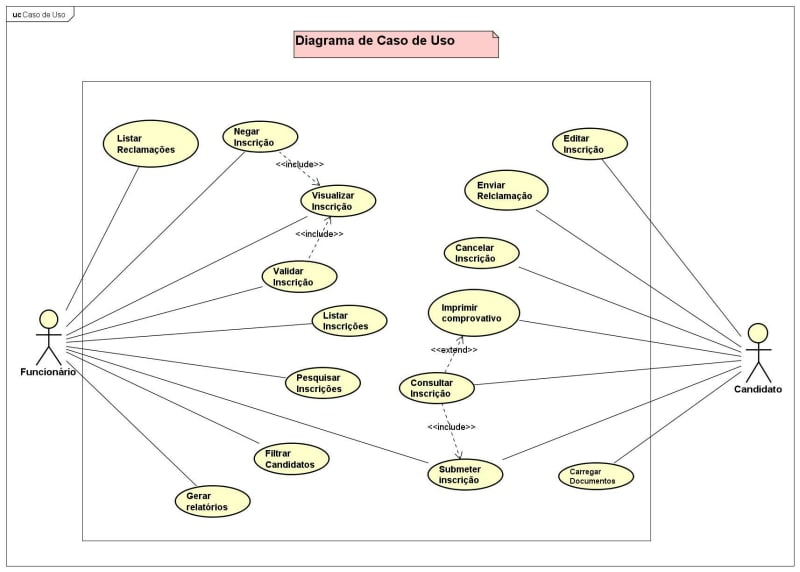
\includegraphics[width=1.1\textwidth]{Logos/caso_de_uso_1.jpg}
\SourceOrNote{Maia (2024)}
\end{figure}

    Não deixe a seção terminar com a imagem então sempre adicione um texto após a mesma.
    
    \subsection*{Diagrama de Classe}
    \addcontentsline{toc}{section}{Diagrama de Classe}

    Esse é um exemplo de diagrama de classe, você deverá descrever os elementos presentes no diagrama (classes e relacionamentos).

    \begin{figure}[h]
\centering
\caption{Diagrama de classe}%
\label{fig:diagrama-classe}
 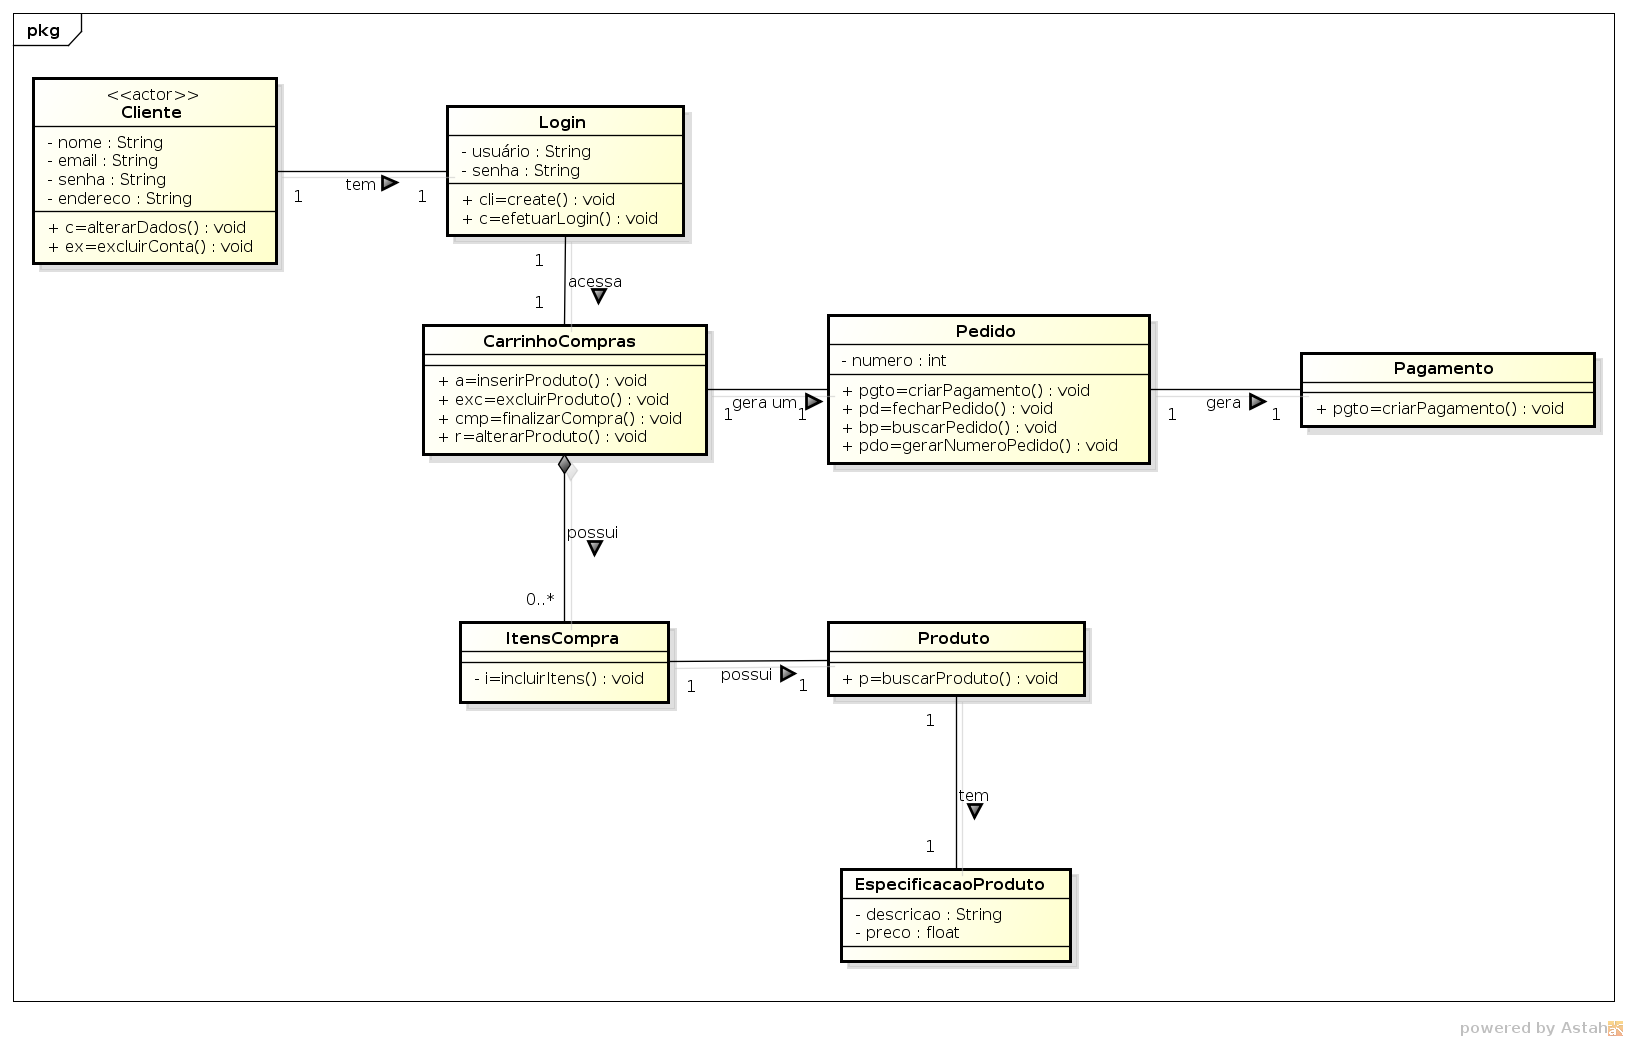
\includegraphics[width=0.8\textwidth]{Logos/diagramaclasse.png}
\SourceOrNote{Maia (2024)}
\end{figure}

     Não deixe a seção terminar com a imagem então sempre adicione um texto após a mesma.

    \subsection*{Diagrama de Objetos}
    \addcontentsline{toc}{section}{Diagrama de Objetos}

Esse é um exemplo de diagrama de objetos.

        \begin{figure}[h]
\centering
\caption{Diagrama de objetos}%
\label{fig:diagrama-objetos}
 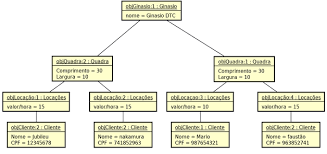
\includegraphics[width=0.8\textwidth]{Logos/diagrama_objetos.png}
\SourceOrNote{Maia (2024)}
\end{figure}

Não deixe a seção terminar com a imagem então sempre adicione um texto após a mesma.

\end{document}